\documentclass[tikz,border=4pt]{standalone}
\usepackage{ctex}
\usepackage{pgfplots}
\pgfplotsset{compat=1.18}
\begin{document}
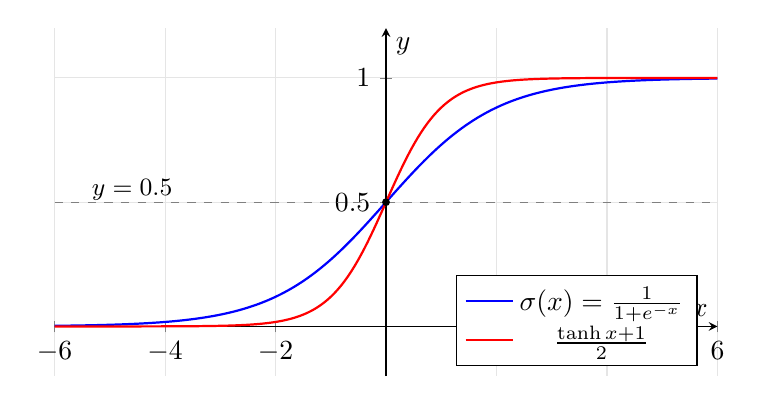
\begin{tikzpicture}
\begin{axis}[
    axis lines=middle, width=10cm, height=6cm,
    xmin=-6, xmax=6, ymin=-0.2, ymax=1.2,
    samples=200, grid=both, grid style={gray!20},
    xlabel={$x$}, ylabel={$y$},
    legend pos=south east,
]
\addplot[blue, thick, domain=-6:6] {1/(1+exp(-x))};
\addlegendentry{$\sigma(x)=\frac{1}{1+e^{-x}}$}
\addplot[red, thick, domain=-6:6] {tanh(x)/2+0.5};
\addlegendentry{$\frac{\tanh x+1}{2}$}
\draw[gray, dashed] (axis cs:-6,0.5) -- (axis cs:6,0.5);
\node[anchor=west] at (axis cs:-5.5,0.55) {\small $y=0.5$};
\node[circle, fill=black, inner sep=1pt] at (axis cs:0,0.5) {};
\end{axis}
\end{tikzpicture}
\end{document}
